% PVLDB research-track paper skeleton.
% Template: PVLDB uses acmart (sigconf, nonacm) with the VLDB header blocks below.
% Before submission, replace the preamble and blocks with the current official template
% from https://vldb.org/pvldb/ and check the current call for papers for the page limit
% (research papers: 12 pages plus references) and the anonymity rules.
%
% Build: tectonic main.tex   (or: latexmk -pdf main.tex)
% Figures are read from ../publication/figures/, so regenerate them there.
% Every number below comes from publication/FULL-RESULTS.md or publication/RELATED-WORK.md;
% the section of FULL-RESULTS each number comes from is given in a comment.

\documentclass[sigconf, nonacm]{acmart}

\usepackage{booktabs}
\usepackage{xcolor}
\graphicspath{{../publication/figures/}}

\newcommand{\todo}[1]{\textcolor{red}{[TODO: #1]}}
\newcommand{\sys}{GPU offload}

%%% VLDB block start %%%
\newcommand\vldbdoi{XX.XX/XXX.XX}
\newcommand\vldbpages{XXX-XXX}
\newcommand\vldbvolume{XX}
\newcommand\vldbissue{X}
\newcommand\vldbyear{2027}
\newcommand\vldbauthors{\authors}
\newcommand\vldbtitle{\shorttitle}
% Leave empty for a double-blind submission; the repository URL identifies the authors.
\newcommand\vldbavailabilityurl{}
\newcommand\vldbpagestyle{plain}
%%% VLDB block end %%%

\begin{document}

% Title options:
%   Whole-Compaction GPU Offload for RocksDB: Compression Included, Shared Across Databases
%   What the CPU Still Does: Offloading All of LSM Compaction, Compression Included, to a GPU
\title{Whole-Compaction GPU Offload for RocksDB: Compression Included, Shared Across Databases}

\author{\todo{Authors}}
\affiliation{\institution{\todo{Institution}}\city{\todo{City}}\country{\todo{Country}}}

\begin{abstract}
Compaction is the largest CPU cost of a write-heavy LSM-tree store. Earlier GPU and FPGA
designs move sorting, merging and block building off the CPU but leave decompression,
compression and checksums on it. Rebuilt inside the same RocksDB and measured on the same
machine, the best of them still uses 49\% of RocksDB's compaction CPU with LZ4 and 69\%
with ZSTD. We offload the whole compaction to a GPU, compression included, while RocksDB
keeps its own file boundaries, index and installation, and we check every compaction's
output against unmodified RocksDB. One compaction runs 8--12$\times$ faster with
9--16$\times$ less CPU for small values, and one GPU does the compaction work of 15--18
cores. With data in memory, the whole database accepts 1.5--1.8$\times$ more writes with
1.8--2.2$\times$ less CPU per write, against 1.14--1.41$\times$ for the earlier designs.
The GPU can be shared: through a compaction service reached over RDMA, eight databases on
another machine each accept 2.1$\times$ RocksDB's writes and keep 89\% of their
throughput alone, with no compaction falling back to the CPU. We also report where the
design does not pay: on a drive that is already the bottleneck, throughput is unchanged and
only the CPU saving and lower tail latency remain; it writes more bytes per user byte; and
at cloud prices it is the cheaper choice only beyond the highest write rate RocksDB can
reach.
\end{abstract}

\maketitle

%%% VLDB block start %%%
\pagestyle{\vldbpagestyle}
\begingroup\small\noindent\raggedright\textbf{PVLDB Reference Format:}\\
\vldbauthors. \vldbtitle. PVLDB, \vldbvolume(\vldbissue): \vldbpages, \vldbyear.\\
\href{https://doi.org/\vldbdoi}{doi:\vldbdoi}
\endgroup
\begingroup
\renewcommand\thefootnote{}\footnote{\noindent
This work is licensed under the Creative Commons BY-NC-ND 4.0 International License. Visit
\url{https://creativecommons.org/licenses/by-nc-nd/4.0/} to view a copy of this license.
For any use beyond those covered by this license, obtain permission by emailing
\href{mailto:info@vldb.org}{info@vldb.org}. Copyright is held by the owner/author(s).
Publication rights licensed to the VLDB Endowment. \\
\raggedright Proceedings of the VLDB Endowment, Vol. \vldbvolume, No. \vldbissue\ %
ISSN 2150-8097. \\
\href{https://doi.org/\vldbdoi}{doi:\vldbdoi} \\
}\addtocounter{footnote}{-1}\endgroup
%%% VLDB block end %%%

%%% VLDB block start %%%
\ifdefempty{\vldbavailabilityurl}{}{
\vspace{.3cm}
\begingroup\small\noindent\raggedright\textbf{PVLDB Artifact Availability:}\\
The source code, data, and/or other artifacts have been made available at
\url{\vldbavailabilityurl}.
\endgroup
}
%%% VLDB block end %%%

% ------------------------------------------------------------------------------------------
\section{Introduction}
\label{sec:intro}

LSM-trees~\cite{oneil1996lsm} accept writes into memory and keep data sorted on storage by
merging files in the background. In RocksDB~\cite{dong2021rocksdb}, this merging,
compaction, is the largest CPU cost of a write-heavy database: with 128-byte values it
takes 3.5--5.5\,\textmu s of CPU per write, more than accepting the write itself
(2.3\,\textmu s). % FULL-RESULTS 3, "Where the CPU goes"
When compaction falls behind, RocksDB slows its writers, and the work it postpones still
has to be done later.

Offloading compaction to an accelerator has been studied for GPUs~\cite{luda2020,glsm2024,
zhou2024msst,gpcomp2025,gclcomp2025,gparakv2025} and FPGAs~\cite{fpga2020}. These designs
take the sort and merge, and in some cases block building, off the CPU. Decompressing the
input and compressing and checksumming the output stay on the CPU. Their published speedups
come from different stores (LevelDB, X-Engine, key-value-separated stores) and different
hardware, so they cannot be compared with each other or with RocksDB.

We rebuilt the two families of earlier designs inside RocksDB~11.8 and measured them on one
machine against the same inputs (Section~\ref{sec:prior}). Offloading sorting and merging
saves little. Offloading everything except decompression, compression and checksums still
leaves 49\% of RocksDB's compaction CPU on the CPU with LZ4 and 69\% with ZSTD.
% RELATED-WORK 1, isolated table: 5.44/11.04 and 14.15/20.46
Since RocksDB normally runs with compression on, compression is most of what the earlier
designs leave behind.

This paper offloads the whole compaction, compression included, and keeps everything that
decides the shape of the LSM-tree in RocksDB. \todo{One paragraph: design summary
(Section~\ref{sec:design}): steps 1--4 on the GPU; RocksDB's own file cuts, index, filter
sizing, properties and installation; logical equivalence checked on every run; eligibility
and CPU fallback; the shared compaction service, local or over RDMA.}

\todo{One paragraph: headline results with the scope stated: in memory; CPU-bound regime;
what changes on drives.}

\paragraph{Contributions.}
\begin{itemize}
  \item A whole-compaction GPU offload inside production RocksDB, including decompression,
        compression, checksums and Bloom-filter hashing, whose output is checked against
        unmodified RocksDB on every run (Sections~\ref{sec:design}, \ref{sec:correct}).
  \item A same-harness evaluation of earlier GPU and FPGA compaction designs, rebuilt in the
        same RocksDB under rules registered before the runs, showing that compression is
        what they leave on the CPU and that without compression the advantage disappears
        (Section~\ref{sec:prior}).
  \item A shared GPU compaction service, reached over shared memory or RDMA, that lets
        several databases use one GPU without CPU fallbacks (Section~\ref{sec:sharing}).
  \item An evaluation with tuned baselines, registered hypotheses and archived data,
        including where the design does not pay: drive-bound systems, write
        amplification, read-heavy work, isolation and cost (Sections~\ref{sec:eval},
        \ref{sec:limits}).
\end{itemize}

\todo{Novelty check before submission: read the full texts of GPComp~\cite{gpcomp2025} and
GCLComp~\cite{gclcomp2025}. If either compresses data blocks on the GPU, the first
contribution becomes ``the first in production RocksDB, measured against the earlier
designs on one harness'', and the introduction must say so.}

% ------------------------------------------------------------------------------------------
\section{Background and Motivation}
\label{sec:background}

\paragraph{Compaction in RocksDB.} \todo{Levelled compaction; the five steps of one
compaction: (1) read and decompress input blocks; (2) merge and drop hidden versions and
obsolete deletions; (3) pack survivors into data blocks; (4) compress and checksum each
block and hash keys for the Bloom filter; (5) cut files, write index, filter, properties
and footer, install the result. Subcompactions; write stalls; postponed compaction.}

\paragraph{Where the CPU goes.} \todo{Use fig39 (CPU per write by job) and the rebuild
ladder of Table~\ref{tab:prior-cpu}: native 11.04 CPU-s/GiB, sort/merge 8.21, pipeline
5.44, ours 2.10 (128\,B, LZ4).}

\paragraph{Earlier accelerator designs.} Table~\ref{tab:designs} summarises what each
family moves off the CPU.

\begin{table}[t]
  \caption{What each design runs on the accelerator.}
  \label{tab:designs}
  \small
  \begin{tabular}{p{0.24\columnwidth}p{0.33\columnwidth}p{0.33\columnwidth}}
    \toprule
    Design (stands in for) & On the accelerator & Left on the CPU \\
    \midrule
    Sort/merge (gLSM~\cite{glsm2024}, gParaKV~\cite{gparakv2025}) & unpack, sort, merge,
      drop hidden versions & decompression, iterator, block building, compression,
      checksums \\
    Pipeline (LUDA~\cite{luda2020}, MSST'24~\cite{zhou2024msst}, FPGA~\cite{fpga2020}) &
      unpack, sort, merge, deletions, block building, filter hashes & decompression,
      compression, checksums \\
    This work & steps 1--4 and Bloom-filter hashing & file cuts, index, metadata, file
      writing \\
    \bottomrule
  \end{tabular}
\end{table}

% ------------------------------------------------------------------------------------------
\section{Design}
\label{sec:design}

\subsection{Offloading a compaction}
\todo{From docs/gpu-compaction.md: per-subcompaction merged input; read into pinned memory;
CRC32C check and nvCOMP~\cite{nvcomp} decode on the device; merge of sorted runs with a
merge-path kernel; hidden-version and deletion rules equal to CompactionIterator without a
SnapshotChecker; block cutting by replaying BlockBuilder's size estimate; nvCOMP LZ4/ZSTD;
masked CRC32C; only finished blocks, boundary keys and filter hashes return to the host.}

\subsection{Keeping RocksDB in charge of the tree}
\todo{RocksDB's own ShouldStopBefore decides file cuts between user keys; built runs are
appended with trailers in pre-reserved gaps; RocksDB chooses filter size and probes, GPU
sets the bits; statistics kept consistent for RocksDB's record-count verification. Why this
matters: the LSM shape and every downstream policy are unchanged.}

\subsection{Eligibility and fallback}
\todo{No merge operator, compaction filter, blob files or range tombstones; format version
6, CRC32C, LZ4/ZSTD/none, keys up to 512 bytes; otherwise RocksDB's own path, with the
reason recorded. GPU out-of-memory: free idle buffers, retry, then fall back.}

\subsection{Remote GPU and the shared compaction service}
\label{sec:design-service}
\todo{One process owns the GPU with K engines; jobs arrive over shared memory or RDMA;
FIFO or per-tenant fair scheduling; on out-of-memory it re-queues instead of failing.
K = 4 chosen by the registered rule (fewest engines within 95\% of the best).}

% ------------------------------------------------------------------------------------------
\section{Correctness}
\label{sec:correct}
Every single-compaction run hashes every stored version (user key, sequence number, type,
value) and the results of 200{,}000 point lookups, which exercise the GPU-built Bloom
filters and indexes, and compares them with unmodified RocksDB. Every whole-database run
checks each read as it happens and every key and value at the end. The GPU code passes
NVIDIA's \texttt{compute-sanitizer} memory, race and synchronisation checks. The output is
logically identical to RocksDB's, not byte-identical: ZSTD output uses nvCOMP's compression
level, so compressed bytes differ while the decompressed data is the same.
% FULL-RESULTS "Correctness"; docs/gpu-compaction.md "Limits"

% ------------------------------------------------------------------------------------------
\section{Evaluation}
\label{sec:eval}

\subsection{Methodology}
\todo{Hardware: server 1 (4$\times$ Xeon Gold 5220, RTX A6000), server 2 (Xeon Silver
4210R, RTX PRO 6000 Blackwell, NVMe), 96-core database machine with 100\,Gb/s RoCE.
RocksDB 11.8; both designs tuned by the same search per core count; fixed-duration runs
(2\,min warm-up, 5\,min measured unless stated) in random order; medians with paired 95\%
bootstrap intervals; hypotheses and thresholds registered before the runs, misses reported;
data in memory unless stated. Workloads: 50\,M keys, 16\,B keys, 128\,B values, batched
writes; YCSB~\cite{cooper2010ycsb}; Meta's models~\cite{cao2020}.}

\subsection{One compaction}
% FULL-RESULTS 1 and 2
\begin{figure}[t]
  \centering
  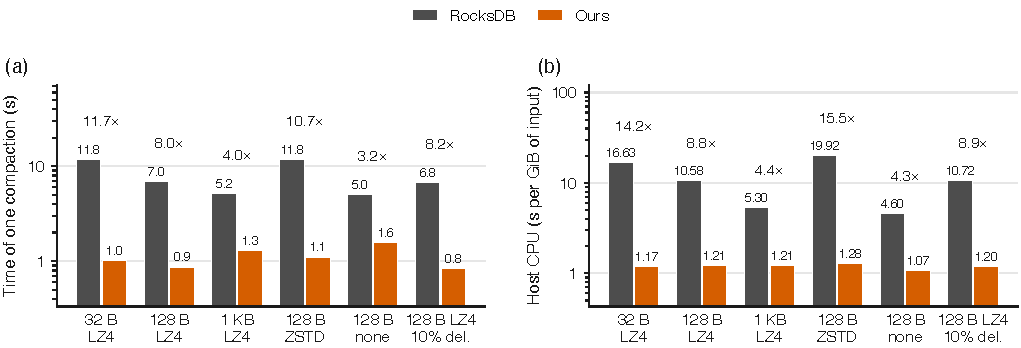
\includegraphics[width=\columnwidth]{fig17_v3_compaction.pdf}
  \caption{One compaction (0.6--0.7\,GiB input): time and CPU per GiB, RocksDB against
  GPU offload. Median of 3 runs, log scale.}
  \label{fig:compaction}
\end{figure}
\todo{8.0--11.7$\times$ faster and 8.8--15.5$\times$ less CPU for 32--128\,B values;
4.0$\times$ / 4.4$\times$ at 1\,KB; 3.2$\times$ / 4.3$\times$ without compression. Ours
stays near 1.2 CPU-s/GiB. Eight concurrent compactions: 1.42\,GiB/s (LZ4) and 0.89\,GiB/s
(ZSTD) using 2.0 and 1.3 cores; one GPU = 15 and 18 RocksDB cores (fig18).}

\subsection{Whole database}
% FULL-RESULTS 3 and 4
\begin{figure}[t]
  \centering
  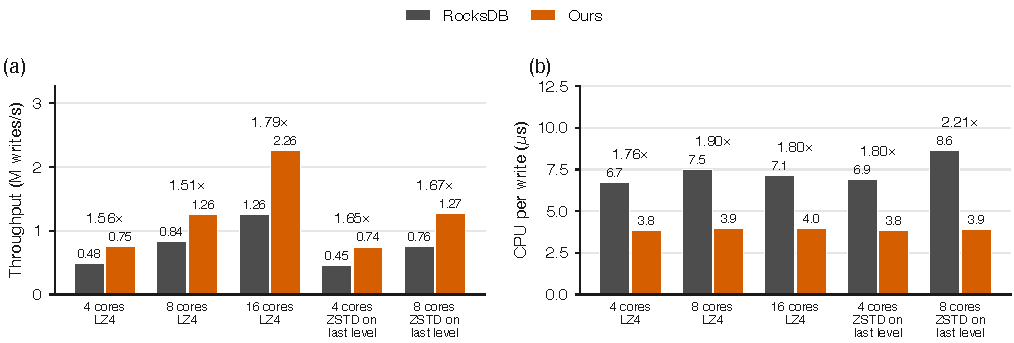
\includegraphics[width=\columnwidth]{fig19_v3_database.pdf}
  \caption{Whole database, 50\,M keys, 128\,B values, batched writes, tuned settings,
  median of 5 runs.}
  \label{fig:database}
\end{figure}
\todo{LZ4: 1.56$\times$ / 1.51$\times$ / 1.79$\times$ more writes at 4 / 8 / 16 cores,
1.76--1.90$\times$ less CPU per write; ZSTD bottom level 1.65--1.67$\times$. No write
stalls (RocksDB up to 6\%). Postponed compaction: RocksDB needs 11--69\,s after 5\,min of
writing, ours 1.3--2.6\,s; counting it, 1.55--1.86$\times$. CPU per write by job (fig39):
compaction 3.5--5.5 to 0.8\,\textmu s; accepting writes unchanged at 2.3\,\textmu s, which
bounds the whole-database gain near 2$\times$.}

\subsection{Tail latency at fixed load}
\todo{Open loop, 8 cores (fig20): p99.9 1.75$\times$ lower at 50\% of RocksDB's maximum
(registered 2.5$\times$ not met), 3.8$\times$ at 70\%, 9.6$\times$ at 90\%.}

\subsection{Earlier designs on the same harness}
\label{sec:prior}
\begin{table}[t]
  \caption{Compaction CPU per GiB of input for one compaction, median of 3 warm runs
  (lower is better). Rebuilds of earlier designs in the same RocksDB.}
  \label{tab:prior-cpu}
  \small
  \begin{tabular}{lrrrr}
    \toprule
    Workload & RocksDB & Sort/merge & Pipeline & Ours \\
    \midrule
    32\,B, LZ4        & 16.93 & 12.40 &  6.08 & \textbf{2.31} \\
    128\,B, LZ4       & 11.04 &  8.21 &  5.44 & \textbf{2.10} \\
    1\,KB, LZ4        &  5.69 &  4.58 &  3.92 & \textbf{1.96} \\
    128\,B, ZSTD      & 20.46 & 17.32 & 14.15 & \textbf{2.19} \\
    128\,B, none      &  5.10 &  3.44 &  1.81 & \textbf{1.80} \\
    \bottomrule
  \end{tabular}
\end{table}
\todo{How the rebuilds work and why they are generous (4 parallel decompression threads,
our GPU sort for LUDA). Whole database, 4 cores (fig36): LZ4 1.14 / 1.41 / 1.75$\times$,
ZSTD 1.16 / 1.17 / 2.27$\times$, none 0.98 / 1.34 / 1.40$\times$. With all designs tuned
(LZ4, 4 cores): 498k / 592k / 756k writes/s. Without compression ours equals the pipeline
design (H8). gParaKV's and LUDA's own code: different stores, reported separately.}

\subsection{Workloads}
\todo{fig32: write-heavy workloads 1.30--1.77$\times$; Meta's ZippyDB model 1.05--1.10$\times$
(85\% reads), write-heavy variant 1.34--1.70$\times$; shared machine (40\% / 80\% of each
core used by another program) 2.14$\times$ / 2.48$\times$; compaction settings (fig40).}

\subsection{Storage}
% FULL-RESULTS 8
\begin{figure}[t]
  \centering
  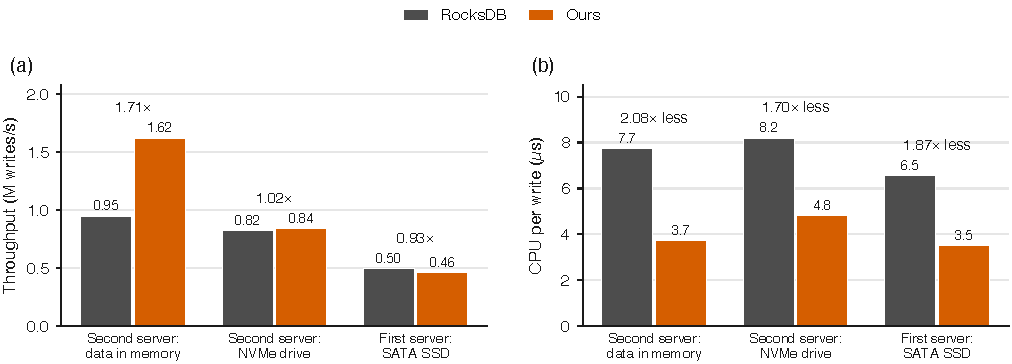
\includegraphics[width=\columnwidth]{fig33_storage.pdf}
  \caption{Throughput and CPU per write in memory, on NVMe (server 2) and on a SATA SSD
  (server 1), 8 cores.}
  \label{fig:storage}
\end{figure}
\todo{When the drive is the limit, throughput is equal: 1.02$\times$ on NVMe, 0.93$\times$
/ 1.04$\times$ on SATA at 8 / 16 cores. CPU per write 1.70$\times$ (NVMe) and
1.87--2.0$\times$ (SATA) lower. NVMe at 630k writes/s: p99 17 vs 503\,ms. At 4 cores on
NVMe, where the CPU is the limit: 1.43$\times$ (2 runs per design; \todo{extend to 5}).
On NVMe ours keeps the drive 89--90\% busy against 55\% because it writes more bytes per
user byte (5.5 vs 4.0); see Section~\ref{sec:limits}.}

\subsection{Remote GPU over RDMA}
\todo{fig31: one compaction 4.0--6.5$\times$ faster than local RocksDB, 5.6--11$\times$
less database-machine CPU; transfer about 0.2\,s of 0.9--1.1\,s. Whole database 802k vs
459k writes/s (1.75$\times$), 2.04$\times$ less CPU per write (1.84$\times$ including the
GPU server). Remote CPU compaction server: same CPU saving, 9.6--17.6\,s per compaction.}

\subsection{Several databases on one GPU}
\label{sec:sharing}
\begin{figure}[t]
  \centering
  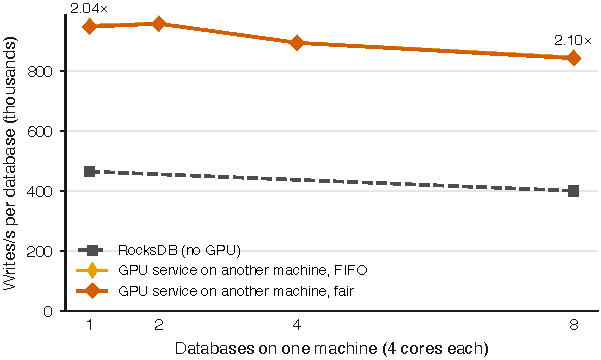
\includegraphics[width=0.8\columnwidth]{fig44_sharing_remote.pdf}
  \caption{Writes/s per database with 1 to 8 databases (4 cores each) sharing one remote
  GPU through the compaction service. Median of 3 runs.}
  \label{fig:sharing}
\end{figure}
\todo{Remote: 8 databases each 842k vs 401k (2.10$\times$), 89\% of solo; 6.7M total;
0 CPU fallbacks; service used 1.9 of 4 cores. Local: 4$\times$8 cores 1.36--1.42$\times$
each; service vs CUDA MPS~\cite{cudamps} within run-to-run variation; without the service
up to 158 CPU fallbacks in 3 runs, MPS up to 124, service 0 in 105 runs; slowest/fastest
0.87--0.91 vs 0.65--0.73 with MPS. Isolation is not provided (Section~\ref{sec:limits}).}

\subsection{Cost}
% FULL-RESULTS 7 and 11; prices.json
\todo{GPU priced as the cheapest AWS GPU with at least the measured card's memory and
bandwidth (A6000 as L40S, \$1.68/h; RTX PRO 6000 as itself, \$3.01/h). Highest rate each
reaches: 2.26M writes/s on 16 cores + GPU at \$0.38 per billion vs RocksDB's 1.60M on 32
cores at \$0.50 (23\% less; break-even GPU price \$2.61/h). Same rate (1.26M): ours 68\%
more (break-even \$0.71/h). Shared remote GPU, 8 databases: 4\% more than RocksDB
(break-even \$2.79/h). Report break-even prices so readers can apply their own.}

% ------------------------------------------------------------------------------------------
\section{Limitations}
\label{sec:limits}
\todo{Drive-bound systems (throughput equal, CPU and tail latency gains remain); write
amplification about 1.4$\times$ higher, all of it compaction output; main cause is eager
level-0 compaction (ours keeps 5.6 vs 9.4 level-0 files and rewrites each write 8.69 vs
6.37 times; raising ours' trigger from 4 to 24 lowers its WA from 6.36 to 3.09 in memory);
about 13\% unexplained, possibly block-granular file cuts (publication/WRITE-AMPLIFICATION.md;
\todo{results of WA-1 and WA-2}); read-heavy work 1.02--1.10$\times$; no compression: no advantage over the
pipeline design; the shared service does not isolate tenants (light tenants 4.2--5.8$\times$
their solo p99.9 next to a heavy one); energy: no general claim (0.69--1.19$\times$ per
write; 1.3--1.5$\times$ lower on a shared machine); cost as above; two GPU models, RocksDB
11.8, one RDMA machine pair; missed registered thresholds listed.}

% ------------------------------------------------------------------------------------------
\section{Related Work}
\label{sec:related}
\paragraph{Accelerated compaction.} \todo{LUDA~\cite{luda2020}, gLSM~\cite{glsm2024},
MSST'24~\cite{zhou2024msst}, GPComp~\cite{gpcomp2025}, GCLComp~\cite{gclcomp2025},
gParaKV~\cite{gparakv2025}, FPGA~\cite{fpga2020}; the NVMe-to-GPU data path line of work
is complementary; concurrent re-evaluation prototype~\cite{reevalgpcomp}.}
\paragraph{Remote and disaggregated compaction.} \todo{Nova-LSM~\cite{novalsm2021},
dLSM~\cite{dlsm2023}, CaaS-LSM~\cite{caaslsm2024}; replication without repeated
compaction: Tebis~\cite{tebis2022}, RubbleDB~\cite{rubbledb2023}. None uses a GPU or
shares one between databases.}
\paragraph{Key-value separation.} \todo{gParaKV compacts fewer bytes by keeping values out
of the sorted files; complementary.}

% ------------------------------------------------------------------------------------------
\section{Conclusion}
\label{sec:conclusion}
\todo{Two or three sentences.}

\bibliographystyle{ACM-Reference-Format}
\bibliography{refs}

\end{document}
